\newpage
\chapter{Simple circuit simulations}
OghmaNano was primarally designed as a tool to perform detailed device simulations, however sometimes one does not need a full device simulation to understand what is happening in your device. On some occasions a simple circuit model comprising of resistors, capacitors, and ideal diodes will do. For these occasions OghmaNano includes an electrical circuit solver. The circuit solver is a drop in replacement for the drift diffusion solver in that the voltages applied to it are defined in exactly defined in exactly the same way, the experimental modes such as time domain, frequency domain and EQE all work with the circuit solver. Furthermore, the transfer matrix model which is used to calculate how much light is absorbed in each layer can connected to the diodes, thus enabling photocurrent to be correctly simulated. There are a few examples if circuit simulations in the mode, these can be found in the \emph{Simple Diode Model} folder of the new simulation folder (see figure \ref{fig:circuit_new_device}.).

\noindent
\begin{minipage}{0.5\textwidth}
	\centering
	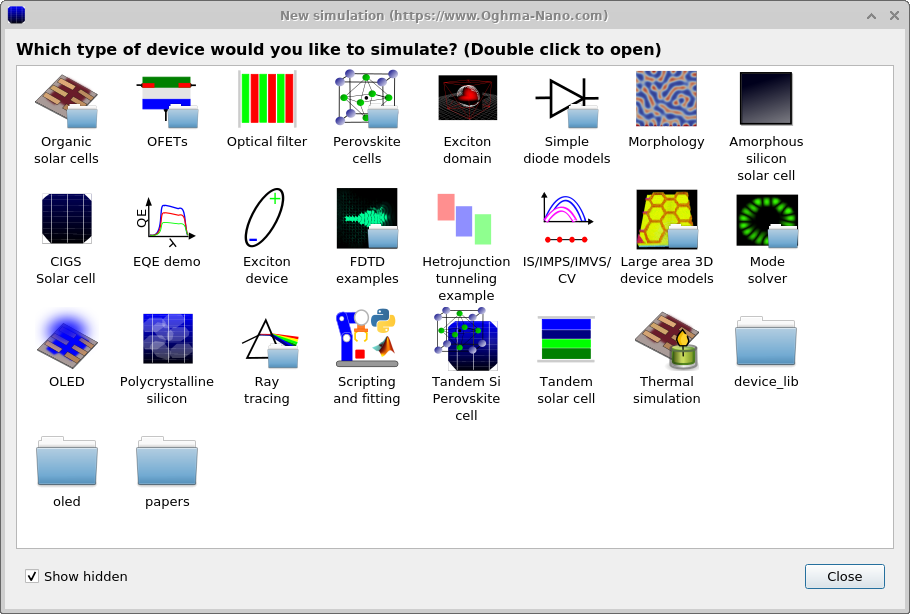
\includegraphics[width=\linewidth,height=0.8\linewidth]{./images/circuit/new_device.png}
	\captionof{figure}{Selecting the \emph{Simple circuit simulation example}}
	\label{fig:circuit_new_device}
\end{minipage}
\hspace{4pt}
\begin{minipage}[]{0.5\linewidth}
	\centering
	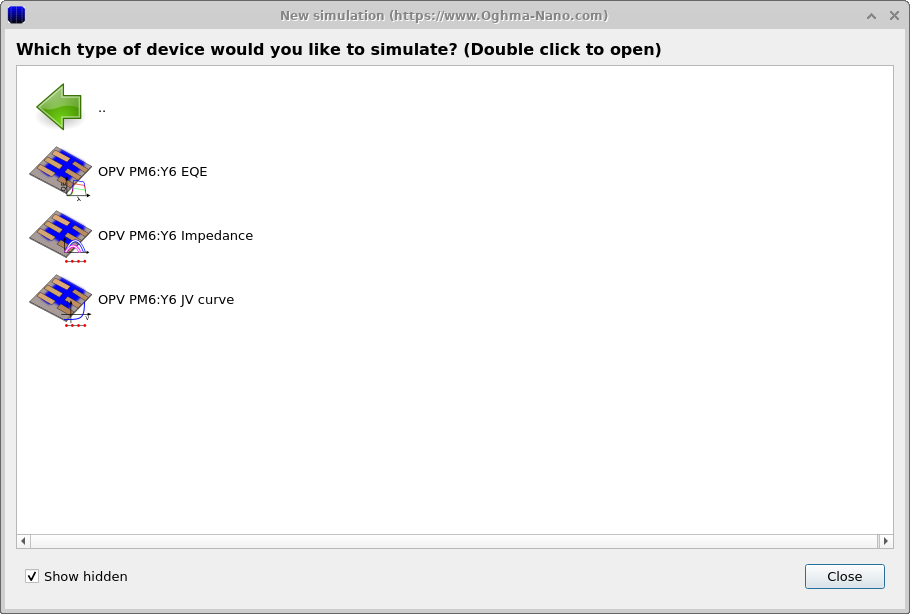
\includegraphics[width=\linewidth,height=0.8\linewidth]{./images/circuit/new_sub_menu.png}
	\captionof{figure}{Selecting the example that generates the JV curve}
	\label{fig:circuit_new_sub_menu}
\end{minipage}

With in this folder there are a few example circuit simulations (see Figure \ref{fig:circuit_new_sub_menu}).

If one opens the \emph{OPV PM6:Y6 JV curve} one will get a simulation that looks just like other simulations in OghmaNano (see Figure \ref{fig:circuit_new_sub_menu}), however this simulation has another tab called \emph{circuit diagram} in the main window, if one clicks it one should see a circuit diagram as show in Figure \ref{fig:circuit_example_circuit}. This is the circuit diagram editor. On the left is a toolbar, from the top the toolbar provides the following functionality:

\begin{itemize}
	\vspace{-0.2cm}\item Resistor: This adds a resistor to the circuit.
	\vspace{-0.2cm}\item Capacitor: This adds a capacitor to the circuit.
	\vspace{-0.2cm}\item Diode: This adds a standard diode to the circuit of form $i(t,V)=I_{0}(e^{\frac{qV}{nkT}}-1)-I_{light}$, $I_{light}$ is taken from the optical simulations.
	\vspace{-0.2cm}\item Non-linear element: This adds a non-linear circuit element of form $i(t,V)={\frac{I_{0}*V}{V_{0}+d}}^m$
	\vspace{-0.2cm}\item Wire: A perfect wire with no parasitic parameters.
 	\vspace{-0.2cm}\item Earth: This acts as a ground set at 0V.
 	\vspace{-0.2cm}\item Battery: This applies the voltage to the circuit. The voltage is taken from the contact marked \emph{change} in the contact editor.
 	\vspace{-0.2cm}\item Pointer: This ise used to select and edit circuit elements.
 	\vspace{-0.2cm}\item Brush: This is used to delete circuit elements.
\end{itemize}

\noindent
\begin{minipage}{0.5\textwidth}
	\centering
	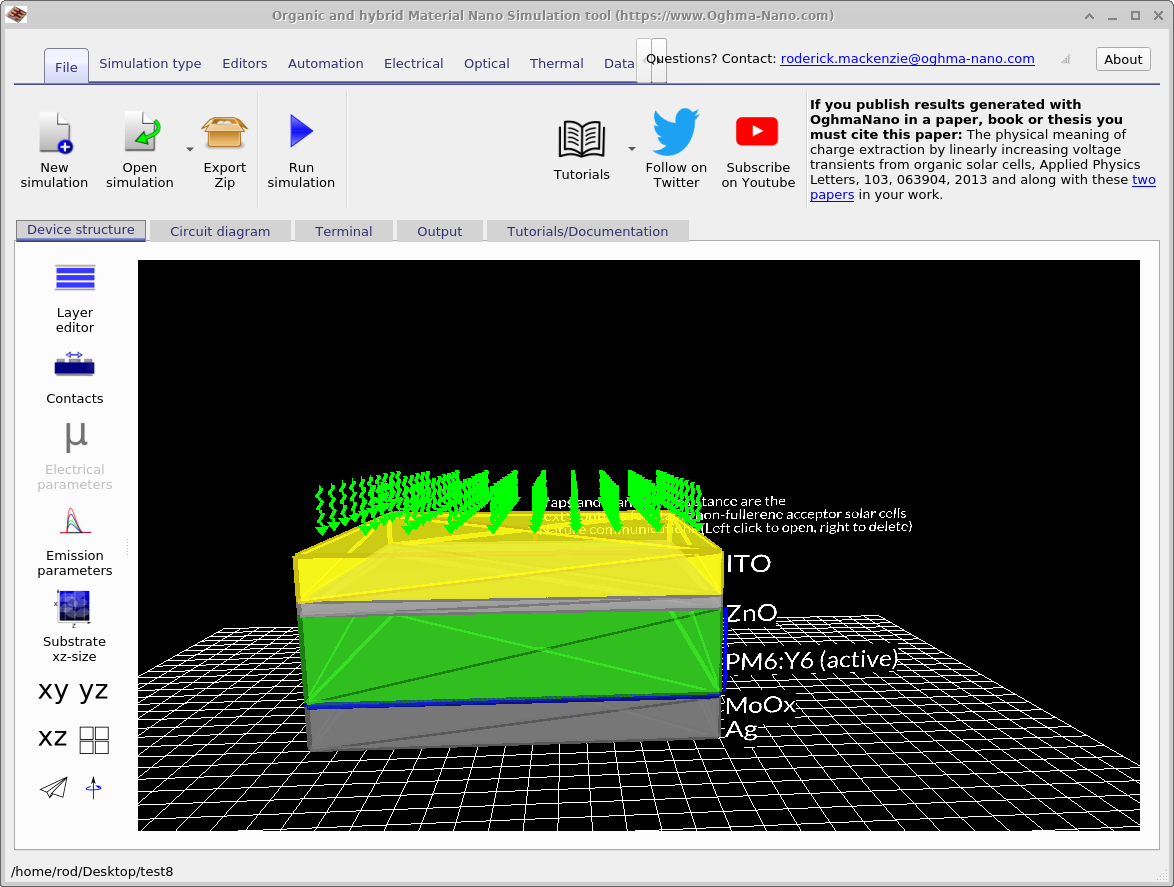
\includegraphics[width=\linewidth,height=0.8\linewidth]{./images/circuit/example_device_sim.png}
	\captionof{figure}{The usual interface opens when the circuit simulation is selected.}
	\label{fig:circuit_example_device_sim}
\end{minipage}
\hspace{4pt}
\begin{minipage}[]{0.5\linewidth}
	\centering
	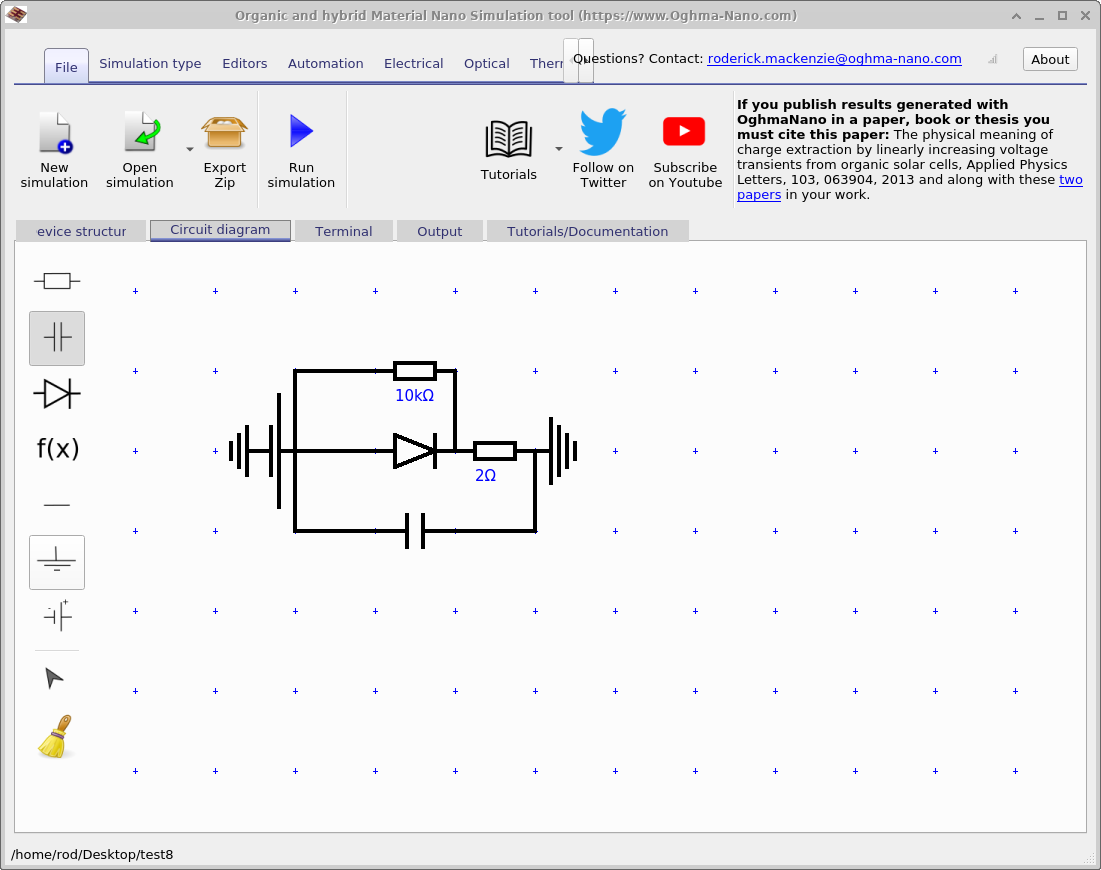
\includegraphics[width=\linewidth,height=0.8\linewidth]{./images/circuit/example_circuit.png}
	\captionof{figure}{The circuit tab of the example showing the circuit diagram used to simulate the device.}
	\label{fig:circuit_example_circuit}
\end{minipage}

By clicking on any circuit element with any tool apart from the brush, you can change the values of the components as seen in Figure \ref{fig:circuit_edit_component}, and zoomed in Figure \ref{fig:circuit_edit_component_zoom}. Figure \ref{fig:circuit_edit_component_zoom} shows the configuration window for the diode component.  From the top the options are:

\begin{itemize}
	\vspace{-0.2cm}\item Component: This can be used to change what component the circuit element represents.
	\vspace{-0.2cm}\item Name: This is an human readable name given to the circuit element, you can call it what you want.
	\vspace{-0.2cm}\item Ideality factor: The diode ideality factor n.
	\vspace{-0.2cm}\item I0: Saturation current in the diode equation.
	\vspace{-0.2cm}\item Layer: This is the layer that the diode represents, the light current will be calculated from the generation in this layer.

\end{itemize}

\noindent
\begin{minipage}{0.5\textwidth}
	\centering
	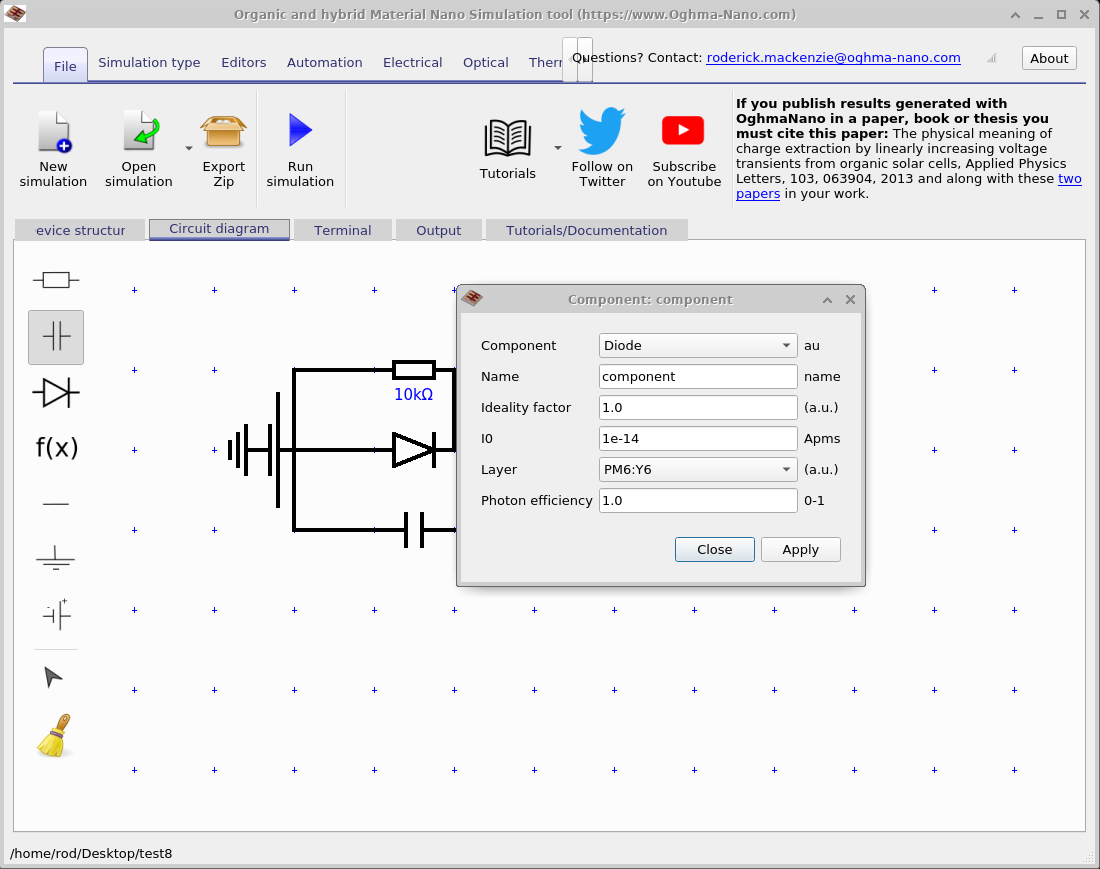
\includegraphics[width=\linewidth,height=0.8\linewidth]{./images/circuit/edit_component.png}
	\captionof{figure}{Editing the component values of a diode.}
	\label{fig:circuit_edit_component}
\end{minipage}
\hspace{4pt}
\begin{minipage}[]{0.5\linewidth}
	\centering
	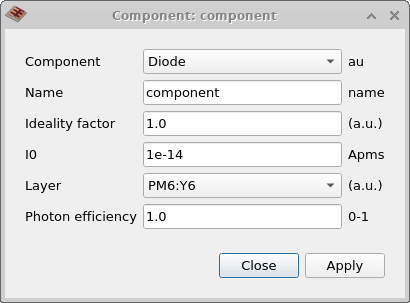
\includegraphics[width=\linewidth,height=0.8\linewidth]{./images/circuit/circuit_edit_component_zoom.png}
	\captionof{figure}{A zoomed in view of the diode component editor. Access this menu by clicking on a component.}
	\label{fig:circuit_edit_component_zoom}
\end{minipage}

After you have run the simulation by clicking the play button or by pressing F9, simulation output will be visible in the output tab as usual.  All the files you would expect from the usual drift diffusion simulations will be generated. One extra output that is generated in the circuit simulation is the \emph{Net list} this is visible in Figure \ref{fig:circuit_net_list}, when you double click on this it brings up the Net list window which is visible in Figure \ref{fig:circuit_net_list}, this shows the voltage over and current through every component in the circuit. You can use the slider to step through the simulation steps, these will be time or voltage steps. The net list is only generated when the simulation output is set to \emph{Write everything to disk} in the simulation editor.



\begin{figure}
\centering
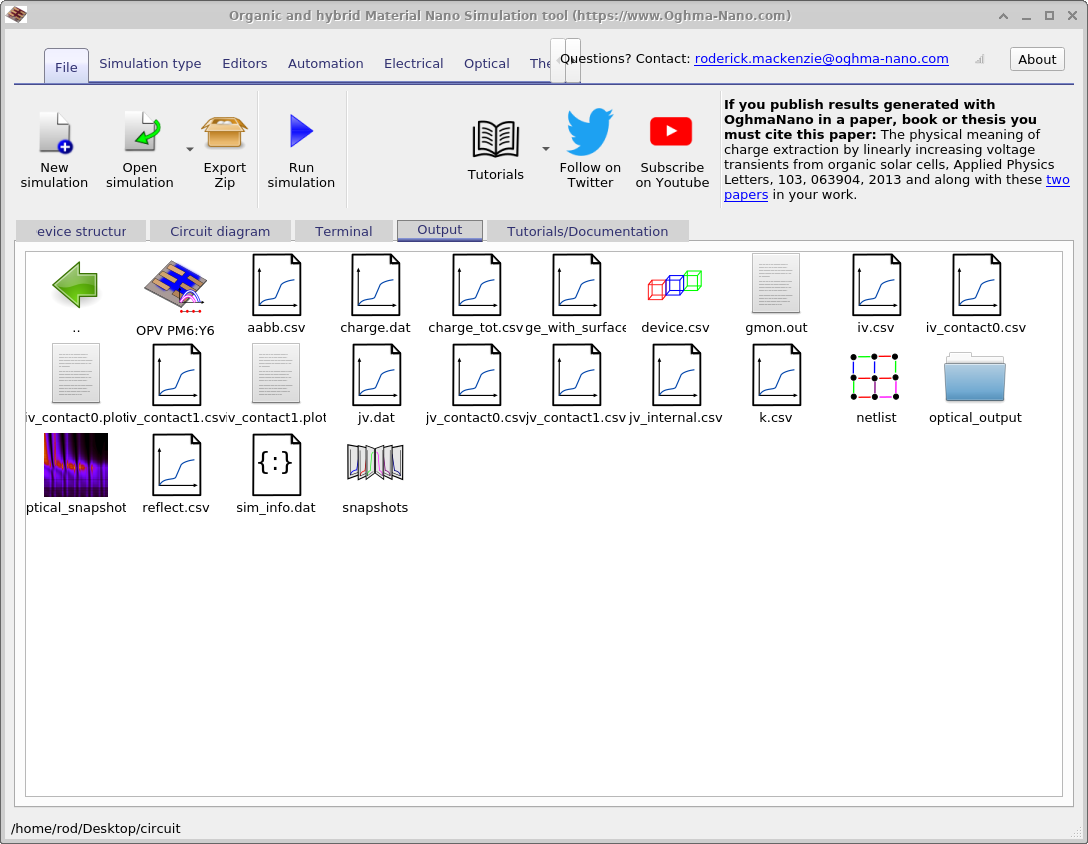
\includegraphics[width=0.7\textwidth,height=0.6\textwidth]{./images/circuit/1.png}
\caption{The output of circuit simulation window is exactly as it would be for standard drift diffusion simulations.}
\label{fig:circuit_1}
\end{figure}

\begin{figure}
\centering
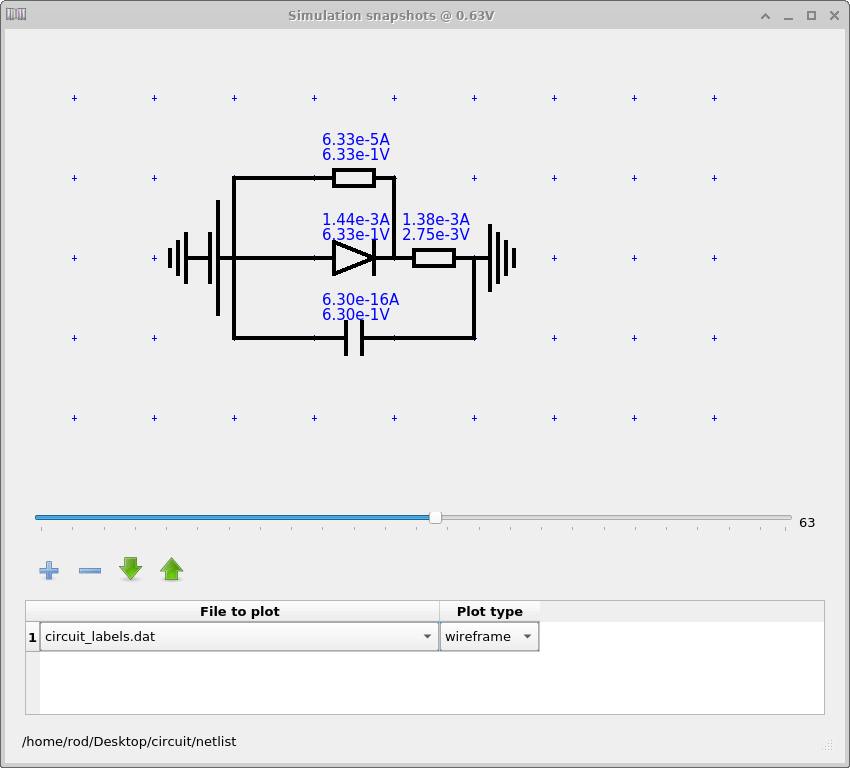
\includegraphics[width=0.7\textwidth,height=0.6\textwidth]{./images/circuit/net_list.png}
\caption{The net list, showing the voltages over components and currents through components.}
\label{fig:circuit_net_list}
\end{figure}

\subsection{JV, IS, CV and other simulation modes}
As mentioned above the circuit simulator is compatible all simulation modes in OghmaNano, by switching the simulation mode to Impedance Spectroscopy one can simulate the frequency response of the circuit (see Figure \ref{fig:simulation_modes}), the result of which can be seen in Figure \ref{fig:circuit_real_imag} where the file real\_imag.csv has been plotted.
 
\begin{figure}[H]
\centering
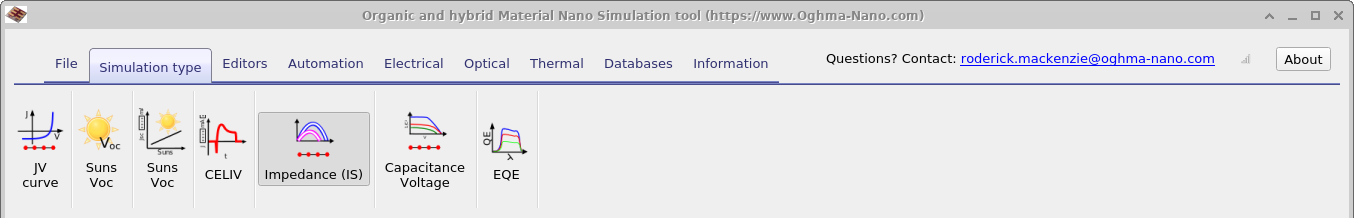
\includegraphics[width=1.0\textwidth,height=0.17\textwidth]{./images/circuit/simulation_modes.png}
\caption{Changing the simulation mode to impedance spectroscopy.}
\label{fig:simulation_modes}
\end{figure}

\begin{figure}[H]
\centering
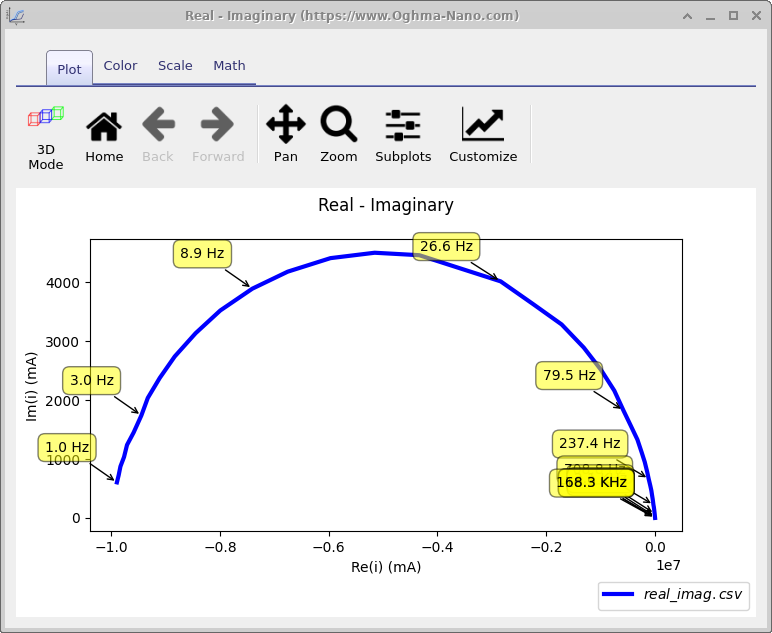
\includegraphics[width=0.7\textwidth,height=0.6\textwidth]{./images/circuit/real_imag.png}
\caption{An impedance spectroscopy simulation performed using the above circuit. To do this just change the simulation mode to IS.}
\label{fig:circuit_real_imag}
\end{figure}

\subsection{Using the fitting/scan tools with circuit models}
The circuit models are exposed in the json tree just like the drift diffusion material paramters and therefore you can also use the fitting and scan tools to either fit the data to experiment or to scan through circuit values.

